%Conclusion body
%Created MB 04-12

\section{Analysis}\label{analysis}
\subsection{Second Sound Analysis}\label{analysis}

By analyzing the second sound data shown in Figure \ref{fig:secondsoundraw}, we can determine the relationship between the temperature of He II and the propagation speed of second sound.  By using linear regression analysis, we can determine the slope of each temperature data set.  For each of the fifteen data sets, the coefficient of determination, $r^{2}$ is greater than $0.99$.  The values for the slope of these fits, in m/s, correspond to the propagation speed of second sound in the respective temperature.  These speeds can then be plotted against temperature in order to show the relationship between the two in He II.  Due to the goodness of each fit, the statistical error in the data is smaller than each speed's level of precision. Figure \ref{fig:secondsound} shows the relationship between second sound speed and temperature in He II.  This data is compared to results made by Peshkov.\cite{peshkov}

\begin{figure}[htbp]
\begin{center}
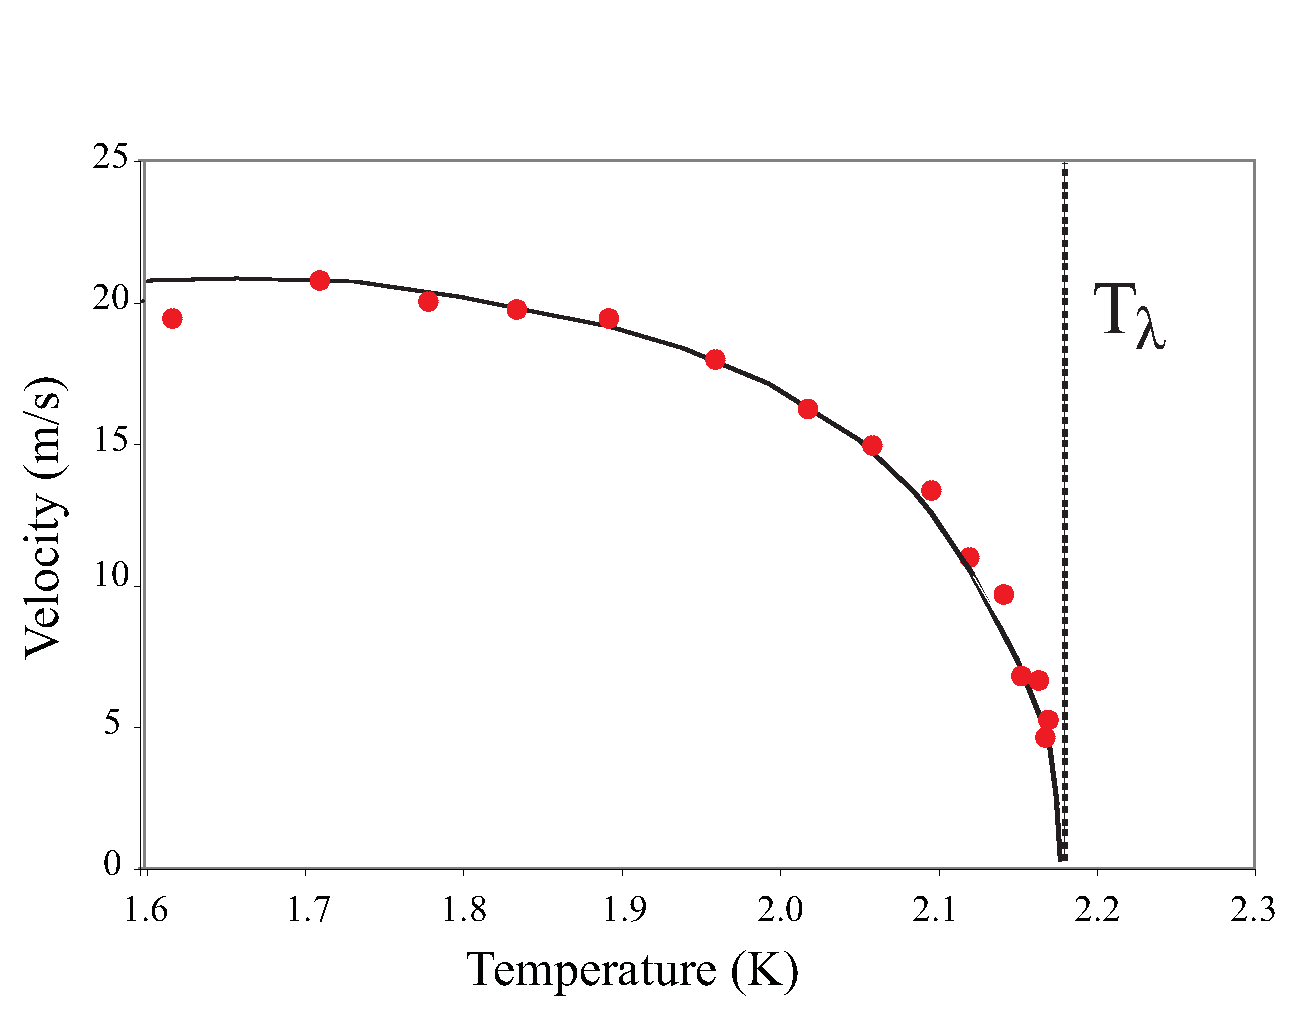
\includegraphics[height=70mm]{./figures/secondsound.eps}
\caption{\small{A plot of the second sound speed verses temperature in He (II).  This data is compared to Peshkov's results.\cite{peshkov} Second sound velocity goes to zero at the transition from He (II) to He (I) enabling a rough estimate of $T_{\lambda}$.}}
\label{fig:secondsound}
\end{center}
\end{figure}

In order to eliminate systematic error in second sound calculations, we chose not to calculate velocity by simply dividing a measured displacement between the balometer from the heater by an observed time delay between the pulse trigger and signature recorded by the balometer. This method would insert systematic offsets to either the time delay or the displacement which would then affect the overall accuracy of second sound speeds.  By calculating the slope of several of these measurements we remove the effect of these offsets and instead emphasize the relative differences between data points.  As a result, the error in second sound speed is purely statistical given by the linear regression analysis.  

\subsection{Heat Capacity Analysis}\label{heatcapacityanalysis}
\subsubsection{Temperature Calibration}\label{temperaturecalibration}

In order to measure heat capacity, we must be able to measure the temperature of the cell.  Because the germanium resistor is thermally coupled to the cell, we can use it as a thermometer for the cell.  Thus the potential difference across the resistor must be converted to temperature.  Following the procedure described in Section \ref{heatcapacityexperiment}, data relating the potential difference across the resistor to the temperature of the cell is produced.  This data can then be fit to a curve given by Equation \ref{eq:fiteqn} in order to determine an expression for temperature as a function of electric potential.  This data with the fit is shown in Figure \ref{fig:polyfit}.  

\begin{figure}[htbp]
\begin{center}
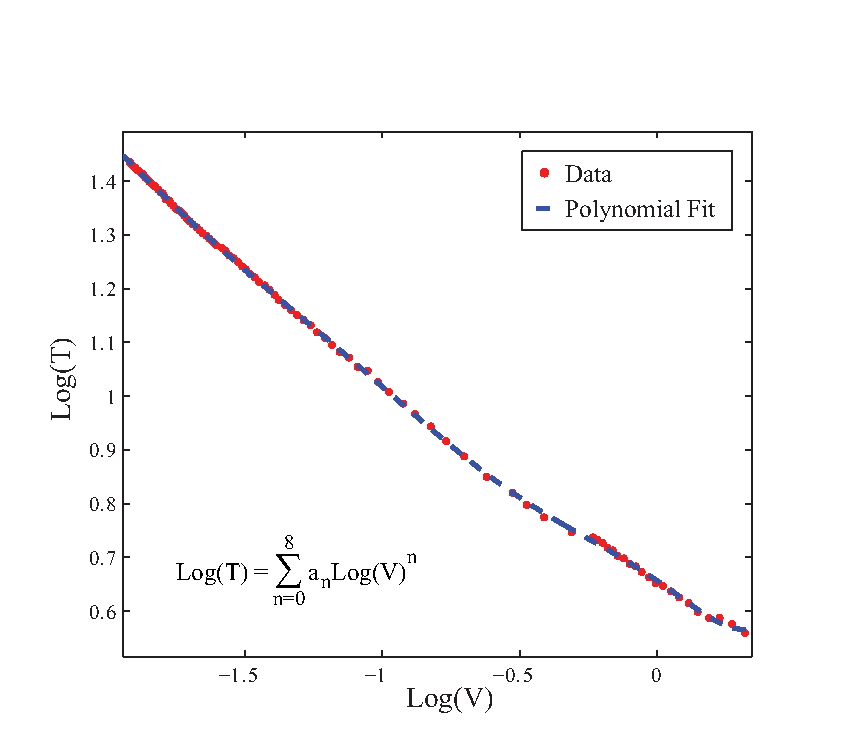
\includegraphics[height=70mm]{./figures/polyfit.eps}
\caption{\small{This plot show the log-log relationship between the potential difference across the germanium resistor and the temperature of the cell for temperatures ranging between $1.8$ K and $4$ K.  The fit is based on Equation \ref{eq:fiteqn} resulting in an $8^{th}$-degree polynomial using nonlinear regression analysis.  The resultant $r^{2}$ value is $0.999$.}}
\label{fig:polyfit}
\end{center}
\end{figure}

The fit was computed doing a $8^{th}$-degree polynomial regression of the log-log data and found to be 

\begin{center}
\begin{equation}\label{eq:polyfit}
ln(T) = 0.6568 - 0.3503ln(V) - 0.1635ln(V)^{2} + 0.2846ln(V)^{3} + 1.813ln(V)^{4} + 2.521ln(V)^{5} + 1.593ln(V)^{6} + 0.4845ln(V)^{7} + 0.0578ln(V)^{8}
\end{equation}
\end{center}
where $T$ is the temperature of the cell and $V$ is the potential difference across the germanium resistor.  Relative uncertainties in the fitting parameters of this polynomial will add to the relative error in calculated temperatures.   

\subsubsection{Calculating the Heat Capacity of Helium}\label{calculatingtheheatcapacityofthecell}

In order to calculate heat capacity from the data shown in Figure \ref{fig:rawdata}, the potential difference across the germanium resistor must be converted to temperature using Equation \ref{eq:polyfit} determined in Section \ref{temperaturecalibration}. A portion of the sample data after being converted from potential to temperature is shown in Figure \ref{fig:heatingdata}.  

\begin{figure}[htbp]
\begin{center}
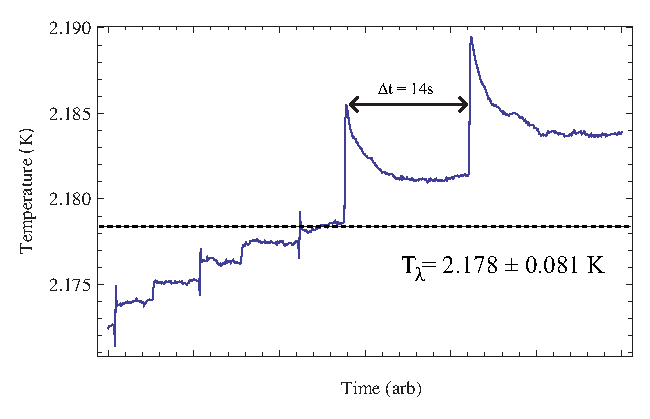
\includegraphics[height=70mm]{./figures/heatingdata.eps}
\caption{\small{A plot of the data from Figure~\ref{fig:rawdata} (b) after being converted from electric potential to temperature using the calibration in Section \ref{temperaturecalibration}.  From this data, $T_{\lambda}$ is determined to be $2.178\pm0.081$ K.}}
\label{fig:heatingdata}
\end{center}
\end{figure}

By analyzing data shown in Figure \ref{fig:rawdata} (b) and using Equation \ref{eq:polyfit}, we can determine the value for $T_{\lambda}$ from $V_{\lambda}$, which is defined as the potential difference across the germanium resistor at which which the He within the cell transitions form a superfluid to a fluid. 

As the temperature of He II heats to $T_{\lambda}$, the change in temperature, $\Delta T$, decreases for a constant heat pulse $Q$.  This implies the change in electric potential, $\Delta V$, decreases as it heats to $V_{\lambda}$.  The transition from He I to He II is denoted by a change in the heat pulse's signature.  As seen in Figure \ref{fig:rawdata}, $\Delta V$ transitions from discrete steps to discrete exponentially decaying steps.  This signature is repeated after converting electric potential to temperature as shown in Figure \ref{fig:heatingdata}.  The reason for this change in signature is due to the drastic divergence of the heat capacity of helium at $T_{\lambda}$.  For temperatures less than $T_{\lambda}$, the energy of the heat pulse sent to the cell is immediately absorbed uniformly in the He II due to the inability of superfluids to have temperature gradients.  This is translated to the discrete steps we see in Figures \ref{fig:rawdata} and \ref{fig:heatingdata}.  For temperatures greater than $T_{\lambda}$, the liquid helium, no longer in its superfluid state, can support temperature gradients.  As a result, the heat pulse is not immediately absorbed by the helium.  Instead the time constant describing the transfer of heat from the Cu addendum to the contained helium is much longer due to the He I's ability to support temperature gradients. This results in a clearly exponential cooling curve as we see in Figures \ref{fig:rawdata} and \ref{fig:heatingdata}.  

From this analysis, we can determine the range in which $T_{\lambda}$ occurs, namely between the temperatures which we know correspond to either He I or He II.  More precisely, we know that a heat pulse followed by discrete step in electric potential (or temperature) is the signature of He II.  While an exponentially decaying signature corresponds to He I. Therefore the transition must lie in between these signatures.  Observing our measured electric potential data in Figure \ref{fig:rawdata}, the interval for $V_{\lambda}$ must be as shown.  With Equation \ref{eq:polyfit}, we can convert this potential to temperature in order to determine $T_{\lambda}$.  Figure \ref{fig:heatingdata} shows the interval for $T_{\lambda}$ which we calculate to be $2.176\pm.hdf$. 

To calculate heat capacity we use the converted temperature data in order to determine the cell's change in temperature, $\Delta T$, from some initial temperature T when for each heat pulse with known energy $Q$.  To do this intensive calculation, due to the number of sent heat pulses being quite large ($>500$), we created a \emph{Mathematica} program which would iteratively measure $\Delta T$ over the entire temperature range observed ($>50000$ data points).  By designating a threshold which varies over different temperature regions, the program identifies occurrences of sudden jumps in temperature corresponding to a heat pulse's signature. Having identified a pulse, the steady state mean temperatures before and after the pulse are recorded \footnote{The determination of the steady state temperature varied according to the temperature relative to $T_{\lambda}$.} and $\Delta T$ is computed.  Heat capacity is then calculated for each $\Delta T$ where $C=Q/\Delta T$.  This process produces data relating the heat capacity to temperature.  Using this algorithm, we are able to determine this relationship for both the evacuated and filled Cu addendum (Figure \ref{fig:lambdanorm}).


\begin{figure}[htbp]
\begin{center}
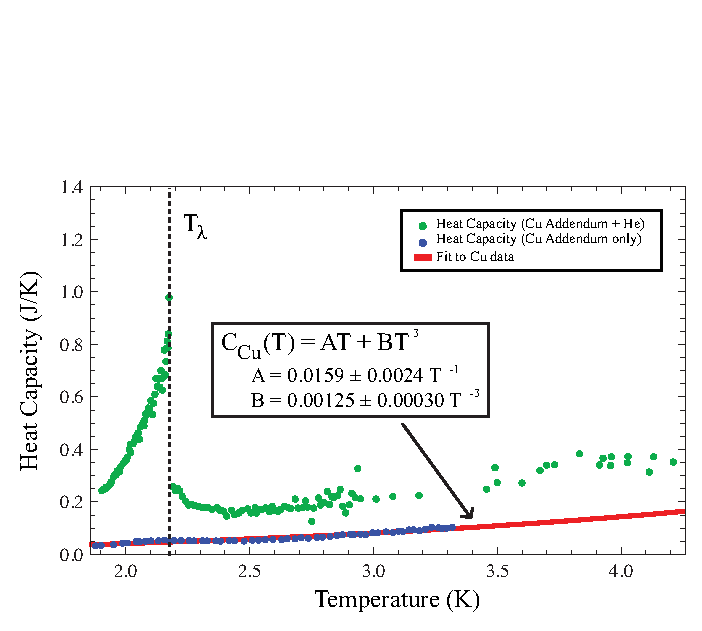
\includegraphics[height=80mm]{./figures/lambdanorm.eps}
\caption{\small{A plot of the heat capacity of the Cu addendum filled with He (II)) and the heat capacity of the evacuated Cu addendum.  A polynomial with cubic and linear terms was fit to the Cu data in order to ultimately remove the addendum's contribution to the heat capacity data.}}
\label{fig:lambdanorm}
\end{center}
\end{figure}

To determine heat capacity of He without the Cu addendum we need to uniformly subtract heat capacity of the Cu addendum from the filled addendum measurement.  To do this we fit a curve to the empty Cu addendum data.  At low temperatures, the heat capacity of copper is dominated by the effect of conduction electrons (which is linear with temperature) and the effect of phonon vibrations (which is cubic with temperature).  Therefore we fit the Cu heat capacity data to a $3^{rd}$-degree polynomial without  quadratic or constant terms using nonlinear regression.  We find that the heat capacity of the Cu addendum is given by

\begin{center}
\begin{equation}\label{eq:cufit}
C^{Cu}_{p} =( 0.0159\pm0.0024 K^{-1}) T + (0.00125\pm0.00030 K^{-3}) T^{3} 
\end{equation}
\end{center}

To remove the Cu addition to the combined heat capacity at a specific temperature, we simply subtract the heat capacity of Cu, given by Equation \ref{eq:cufit}, for that temperature. Thus we are able to calculate the heat capacity of the He which is contained in the cell for the temperature region observed.  This heat capacity data must then be normalized to account for the amount of He in the cell. As described in Section \ref{heatcapacityexperiment}, by measuring the pressure of a certain volume of He at room temperature, we can use the ideal gas law to compute the number of moles of He in that volume.  That volume is then inserted into the cell through a capillary tubing.  We assume that almost all of the He is condensed in the cell due to the density of liquid helium being much greater than that of gaseous helium.  Knowing the number of moles of He in the cell, we can calculate its specific heat in J/mol K. This final data is shown in Figure \ref{fig:lambdatrans}.

\begin{figure}[htbp]
\begin{center}
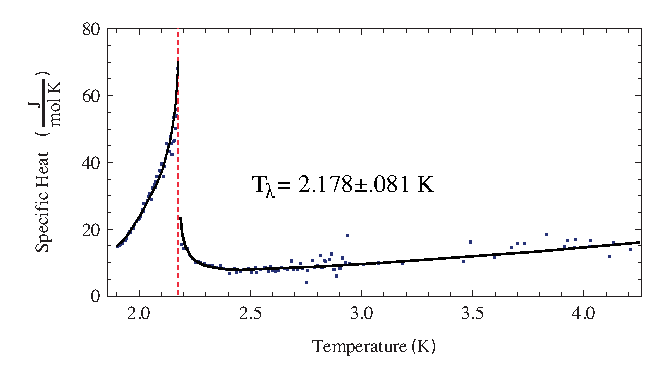
\includegraphics[height=80mm]{./figures/lambdatrans.eps}
\caption{\small{A plot of the specific heat of He(II) verses temperature. The transition from He(I) to He (II) occurs at $T_{\lambda} = 2.178 \pm .081$ K.  The values for specific heat each have a statistical error of $Blah$ J/mol K.}}
\label{fig:lambdatrans}
\end{center}
\end{figure}

